\chapter{Electronegativity, Polarity and Intermolecular Forces}\label{ch:g11:polarity-and-cohesion}

A gecko runs up a window pane and hangs from the glass by a single toe,
with no glue and no suction cup. A water \omterm{def:g7:atoms-and-molecules:molecule}{molecule}, \ce{H2O}, is lighter
than a \omterm{def:g7:atoms-and-molecules:molecule}{molecule} of hydrogen sulfide, \ce{H2S}, yet water boils at
\qty{100}{\celsius} while hydrogen sulfide is a gas down to
\qty{-60}{\celsius}. Both stories are about the same thing: the forces
that hold \omterm{def:g7:atoms-and-molecules:molecule}{molecules} to one another, and to other things. They are far
weaker than the \omterm{def:g10:lewis-and-shape:covalent-bond}{covalent bonds} inside a \omterm{def:g7:atoms-and-molecules:molecule}{molecule}, but they decide whether
a substance is a gas, a liquid or a solid at room temperature, and
whether a gecko falls.

\begin{recall}
A \omterm{def:g10:lewis-and-shape:covalent-bond}{covalent bond} is a pair of \omterm{def:g9:inside-the-atom:nucleus}{electrons} shared by two \omterm{def:g7:atoms-and-molecules:atom}{atoms}; \omterm{def:g10:lewis-and-shape:lewis-structure}{Lewis
structures} show \omterm{def:g10:lewis-and-shape:lone-pair}{bonding pairs} and \omterm{def:g10:lewis-and-shape:lone-pair}{lone pairs}, and the pairs around a
central \omterm{def:g7:atoms-and-molecules:atom}{atom} decide the shape of a \omterm{def:g7:atoms-and-molecules:molecule}{molecule}
(\cref{ch:g10:lewis-and-shape}). \omterm{def:g9:ions:ion}{Ions} carry a charge; in an ionic solid,
positive and negative \omterm{def:g9:ions:ion}{ions} attract one another (\cref{ch:g9:ions}).
\end{recall}

\begin{omfigure}
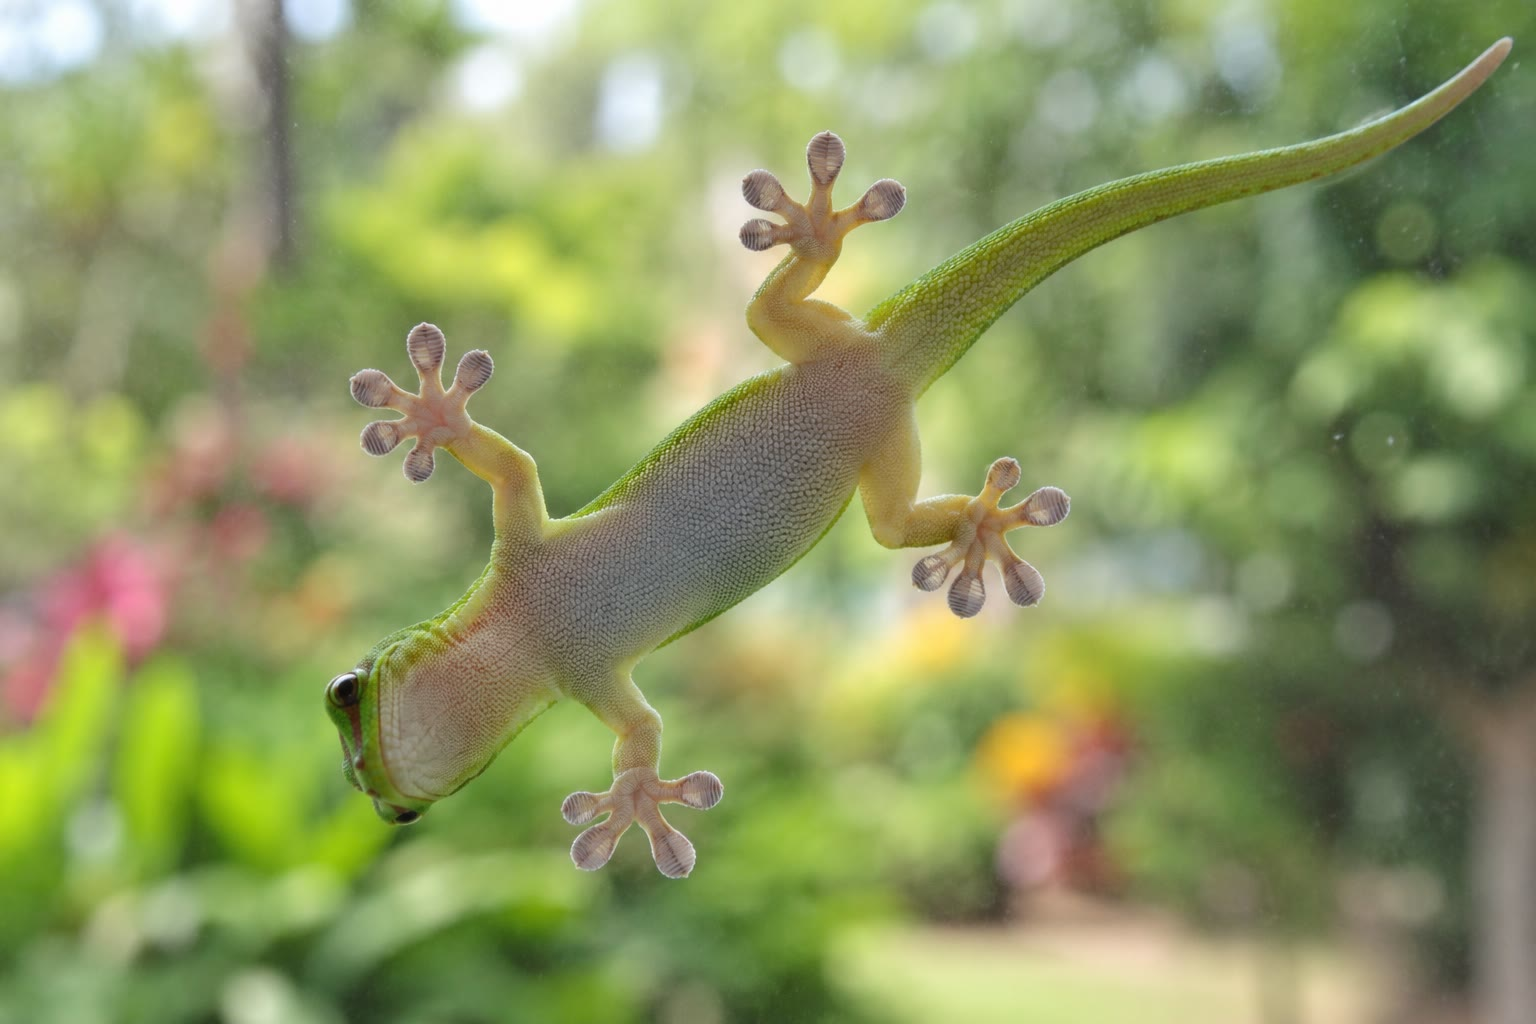
\includegraphics[width=0.5\linewidth]{images/book1/ai/g11-gecko-glass.jpg}

{\small A gecko on a glass pane: its toe pads hold by forces between
\omterm{def:g7:atoms-and-molecules:molecule}{molecules}.}
\end{omfigure}

\section{Electronegativity}

\begin{definition}[Electronegativity]\label{def:g11:polarity-and-cohesion:electronegativity}
The \emph{electronegativity}\index{electronegativity} of an element
measures how strongly its \omterm{def:g7:atoms-and-molecules:atom}{atoms}, in a \omterm{def:g7:atoms-and-molecules:molecule}{molecule}, attract the \omterm{def:g9:inside-the-atom:nucleus}{electrons} of
the bonds they share. It is a number without unit; on the usual scale it
runs from about 0.8 to about 4.
\end{definition}

\begin{omfigure}
% ledger: en:H, en:Li, en:Be, en:B, en:C, en:N, en:O, en:F, en:Na, en:Mg, en:Al, en:Si, en:P, en:S, en:Cl, en:K, en:Ca
\omperiodictable[upto=20, f block=false, cell=0.9cm, values={H/2.20,
  Li/0.98, Be/1.57, B/2.04, C/2.55, N/3.04, O/3.44, F/3.98, Na/0.93,
  Mg/1.31, Al/1.61, Si/1.90, P/2.19, S/2.58, Cl/3.16, K/0.82, Ca/1.00},
  highlight={F,O,N,Cl}]

{\small Electronegativities of the first twenty elements (Pauling scale;
none is given for helium, neon and argon, which form no bonds here).
Highlighted: the four most electronegative.}
\end{omfigure}

\begin{proposition}[Trends in the table]\label{prop:g11:polarity-and-cohesion:trends}
% ledger: en:F, en:Li, en:Cl, en:K
\omterm{def:g11:polarity-and-cohesion:electronegativity}{Electronegativity} increases from left to right along a period and
decreases from top to bottom in a group. Fluorine (3.98) is the most
electronegative element; the \omterm{def:g10:electron-shells:family}{alkali metals} are the least (lithium 0.98,
potassium 0.82).
\end{proposition}

\begin{proof}
Read on the table: along period 2, $0.98 < 1.57 < 2.04 < 2.55 < 3.04 <
3.44 < 3.98$; down \omterm{def:g9:periodic-table-first-look:period}{group} 17, fluorine $3.98$ is above chlorine
$3.16$; down \omterm{def:g9:periodic-table-first-look:period}{group} 1, $2.20$, $0.98$, $0.93$, $0.82$. (Why it is so is
explained in the Year 1 volume.)
\end{proof}

\begin{history}[Pauling's scale, 1932]
The chemist Linus Pauling built the first \omterm{def:g11:polarity-and-cohesion:electronegativity}{electronegativity} scale in
1932, from the energies of bonds between different \omterm{def:g7:atoms-and-molecules:atom}{atoms}. He gave
fluorine the largest value, and the scale used in this chapter is still
called after him.
\end{history}

\section{Polar bonds and polar molecules}

\begin{definition}[Polar bond, partial charge]\label{def:g11:polarity-and-cohesion:polar-bond}
A \omterm{def:g10:lewis-and-shape:covalent-bond}{covalent bond} between two \omterm{def:g7:atoms-and-molecules:atom}{atoms} of different electronegativities is a
\emph{polar bond}\index{polar bond}: the shared pair sits closer to the
more electronegative \omterm{def:g7:atoms-and-molecules:atom}{atom}. That \omterm{def:g7:atoms-and-molecules:atom}{atom} carries a small negative
\emph{partial charge}\index{partial charge}, written $\delta^-$, and the
other \omterm{def:g7:atoms-and-molecules:atom}{atom} an equal positive partial charge, $\delta^+$.
\end{definition}

\begin{proposition}[When is a bond polar?]\label{prop:g11:polarity-and-cohesion:polar-bond}
% ledger: en:C, en:H, en:O, en:Na, en:Cl
A bond between two identical \omterm{def:g7:atoms-and-molecules:atom}{atoms} is not polar. Between different
\omterm{def:g7:atoms-and-molecules:atom}{atoms}, the larger the difference of electronegativities, the more polar
the bond; as a rule of thumb, a difference below about 0.4 (such as
\ce{C-H}, $2.55 - 2.20 = 0.35$) is treated as non-polar. When the
difference is very large (such as Na and Cl, $3.16 - 0.93 = 2.23$), the
\omterm{def:g9:inside-the-atom:nucleus}{electrons} are not shared but transferred: the compound is ionic.
\end{proposition}

\begin{proof}
Admitted: it follows from the definition of \omterm{def:g11:polarity-and-cohesion:electronegativity}{electronegativity}, the
thresholds being conventions.
\end{proof}

\begin{definition}[Polar and non-polar molecules]\label{def:g11:polarity-and-cohesion:polar-molecule}
A \omterm{def:g7:atoms-and-molecules:molecule}{molecule} is a \emph{polar molecule}\index{polar molecule} if the
centre of its positive \omterm{def:g11:polarity-and-cohesion:polar-bond}{partial charges} and the centre of its negative
\omterm{def:g11:polarity-and-cohesion:polar-bond}{partial charges} do not coincide; if they coincide, it is a
\emph{non-polar molecule}\index{non-polar molecule}.
\end{definition}

\begin{method}[Is a molecule polar?]\label{met:g11:polarity-and-cohesion:polar}
\begin{enumerate}
  \item Draw the \omterm{def:g10:lewis-and-shape:lewis-structure}{Lewis structure} and find the shape of the \omterm{def:g7:atoms-and-molecules:molecule}{molecule}.
  \item Mark the \omterm{def:g11:polarity-and-cohesion:polar-bond}{polar bonds} with $\delta^+$ and $\delta^-$.
  \item If there is no \omterm{def:g11:polarity-and-cohesion:polar-bond}{polar bond}, the \omterm{def:g7:atoms-and-molecules:molecule}{molecule} is non-polar. Otherwise,
        look at the shape: if the \omterm{def:g11:polarity-and-cohesion:polar-bond}{polar bonds} are arranged symmetrically
        around the centre, their effects cancel and the \omterm{def:g7:atoms-and-molecules:molecule}{molecule} is
        non-polar; if not, it is polar.
\end{enumerate}
\end{method}

\begin{omfigure}
\begin{tikzpicture}[font=\small]
  % water
  \begin{scope}
    \node[aO] (o) at (0,0) {};
    \node[aH] (h1) at (-0.82,-0.6) {};
    \node[aH] (h2) at (0.82,-0.6) {};
    \begin{scope}[on background layer]
      \draw[bond] (o.center) -- (h1.center); \draw[bond] (o.center) -- (h2.center);
    \end{scope}
    \node[omThm] at (0,0.55) {$2\delta^-$};
    \node[omDef] at (-1.22,-0.5) {$\delta^+$};
    \node[omDef] at (1.22,-0.5) {$\delta^+$};
    \fill[omDef] (0,-0.6) circle (0.06);
    \fill[omThm] (0,0) circle (0.06);
    \draw[densely dotted, black!60] (-0.82,-0.6) -- (0.82,-0.6);
    \draw[<-, black!60] (0.08,-0.64) -- (1.55,-1.05) node[right, align=left,
      font=\footnotesize] {centre of\\ the $\delta^+$};
    \node[align=center, anchor=north] at (0,-1.8) {water: bent, \textbf{polar}};
  \end{scope}
  % carbon dioxide
  \begin{scope}[xshift=6cm]
    \node[aO] (o1) at (-1.15,0) {};
    \node[aC] (c) at (0,0) {};
    \node[aO] (o2) at (1.15,0) {};
    \begin{scope}[on background layer]
      \draw[bond, double, double distance=1.6pt] (o1.center) -- (c.center);
      \draw[bond, double, double distance=1.6pt] (c.center) -- (o2.center);
    \end{scope}
    \node[omThm] at (-1.15,0.55) {$\delta^-$};
    \node[omThm] at (1.15,0.55) {$\delta^-$};
    \node[omDef] at (0,0.55) {$2\delta^+$};
    \draw[->, omProp, thick] (-0.25,-0.45) -- (-1.0,-0.45);
    \draw[->, omProp, thick] (0.25,-0.45) -- (1.0,-0.45);
    \node[align=center, anchor=north] at (0,-1.8) {carbon dioxide: linear,\\
      \textbf{non-polar}};
  \end{scope}
\end{tikzpicture}

{\small In water, the bent shape puts the centre of the positive \omterm{def:g11:polarity-and-cohesion:polar-bond}{partial
charges} (between the hydrogen \omterm{def:g7:atoms-and-molecules:atom}{atoms}) below the oxygen \omterm{def:g7:atoms-and-molecules:atom}{atom}: the \omterm{def:g7:atoms-and-molecules:molecule}{molecule}
is polar. In carbon dioxide the two \omterm{def:g11:polarity-and-cohesion:polar-bond}{polar bonds} pull in opposite
directions (arrows) and cancel: the centres of charge coincide on the
carbon \omterm{def:g7:atoms-and-molecules:atom}{atom}.}
\end{omfigure}


\begin{example}[Four molecules]\label{ex:g11:polarity-and-cohesion:four}
Hydrogen chloride \ce{HCl} has one \omterm{def:g11:polarity-and-cohesion:polar-bond}{polar bond} and is polar, chlorine
$\delta^-$. Ammonia \ce{NH3}, a pyramid of three polar \ce{N-H} bonds,
is polar, nitrogen $\delta^-$. Methane \ce{CH4} has only nearly non-polar
\ce{C-H} bonds: non-polar. Tetrachloromethane \ce{CCl4} has four polar
\ce{C-Cl} bonds, but at the corners of a regular tetrahedron: their
effects cancel and the \omterm{def:g7:atoms-and-molecules:molecule}{molecule} is non-polar.
\end{example}

\section{Van der Waals interactions}

\begin{definition}[Van der Waals interaction]\label{def:g11:polarity-and-cohesion:van-der-waals}
A \emph{van der Waals interaction}\index{van der Waals interaction} is a
weak attraction between neighbouring \omterm{def:g7:atoms-and-molecules:molecule}{molecules}, which exists between all
\omterm{def:g7:atoms-and-molecules:molecule}{molecules}, polar or not: the \omterm{def:g9:inside-the-atom:nucleus}{electrons} of each \omterm{def:g7:atoms-and-molecules:molecule}{molecule} are constantly
moving, and the momentary uneven charges of one \omterm{def:g7:atoms-and-molecules:molecule}{molecule} attract those
of its neighbours. Between \omterm{def:g11:polarity-and-cohesion:polar-molecule}{polar molecules}, the permanent \omterm{def:g11:polarity-and-cohesion:polar-bond}{partial
charges} add a further attraction.
\end{definition}


\begin{proposition}[Bigger molecules attract more]\label{prop:g11:polarity-and-cohesion:size}
\omterm{def:g11:polarity-and-cohesion:van-der-waals}{Van der Waals interactions} grow with the size of the \omterm{def:g7:atoms-and-molecules:molecule}{molecules}, that is,
with the number of their \omterm{def:g9:inside-the-atom:nucleus}{electrons}; between similar \omterm{def:g7:atoms-and-molecules:molecule}{molecules}, the
larger ones have the higher melting and boiling temperatures.
\end{proposition}

\begin{proof}
Admitted: a larger \omterm{def:g9:inside-the-atom:nucleus}{electron} cloud is more easily deformed, so its
momentary charges are larger, and it has more contact with its
neighbours.
\end{proof}

\begin{example}[The halogens]\label{ex:g11:polarity-and-cohesion:halogens}
% ledger: bp:F2, bp:Cl2, bp:Br2, bp:I2 (K values converted)
The \omterm{def:g7:atoms-and-molecules:molecule}{molecules} \ce{F2}, \ce{Cl2}, \ce{Br2}, \ce{I2} are all non-polar and
larger and larger. Their boiling temperatures rise with them:
\qty{-188}{\celsius}, \qty{-34}{\celsius}, \qty{59}{\celsius} and
\qty{184}{\celsius}. At room temperature, fluorine and chlorine are
gases, bromine a liquid, iodine a solid.
\end{example}

\begin{remark}[The gecko]\label{rem:g11:polarity-and-cohesion:gecko}
A single \omterm{def:g11:polarity-and-cohesion:van-der-waals}{van der Waals interaction} is tiny, but they add up. The toe
pads of a gecko are covered with a dense carpet of microscopic hairs,
each split into still finer tips, which come close enough to the glass
for \omterm{def:g11:polarity-and-cohesion:van-der-waals}{van der Waals interactions} to act over a very large total area.
\end{remark}

\section{Hydrogen bonds}

\begin{definition}[Hydrogen bond]\label{def:g11:polarity-and-cohesion:hydrogen-bond}
A \emph{hydrogen bond}\index{hydrogen bond} is an attraction between a
hydrogen \omterm{def:g7:atoms-and-molecules:atom}{atom} bonded to a very electronegative \omterm{def:g7:atoms-and-molecules:atom}{atom} (nitrogen, oxygen or
fluorine), which carries a marked $\delta^+$, and a \omterm{def:g10:lewis-and-shape:lone-pair}{lone pair} of another
nitrogen, oxygen or fluorine \omterm{def:g7:atoms-and-molecules:atom}{atom}, often on a neighbouring \omterm{def:g7:atoms-and-molecules:molecule}{molecule}. It
is drawn as a dashed line, and the three \omterm{def:g7:atoms-and-molecules:atom}{atoms} involved are nearly in a
straight line.
\end{definition}

\begin{omfigure}
\begin{tikzpicture}[font=\small]
  % central water molecule and four neighbours, H-bonds dashed
  \newcommand{\water}[4]{% name, x, y, rotation
    \begin{scope}[shift={(#2,#3)}, rotate=#4]
      \node[aO] (#1o) at (0,0) {};
      \node[aH] (#1a) at (-0.6,-0.45) {};
      \node[aH] (#1b) at (0.6,-0.45) {};
    \end{scope}
    \begin{scope}[on background layer]
      \draw[bond] (#1o.center) -- (#1a.center); \draw[bond] (#1o.center) -- (#1b.center);
    \end{scope}}
  \water{m}{0}{0}{0}
  \water{p}{-1.62}{-1.215}{0}
  \water{q}{1.62}{-1.215}{0}
  \water{r}{-1.435}{1.435}{-8.13}
  \water{s}{1.435}{1.435}{8.13}
  % H-bonds: m's H to p's O and q's O; r's and s's H to m's O
  \draw[dashed, omDef, thick] (ma) -- (po);
  \draw[dashed, omDef, thick] (mb) -- (qo);
  \draw[dashed, omDef, thick] (rb) -- (mo);
  \draw[dashed, omDef, thick] (sa) -- (mo);
\end{tikzpicture}

{\small \omterm{def:g11:polarity-and-cohesion:hydrogen-bond}{Hydrogen bonds} (dashed) around a water \omterm{def:g7:atoms-and-molecules:molecule}{molecule} in liquid water:
its two hydrogen \omterm{def:g7:atoms-and-molecules:atom}{atoms} bond to the oxygen \omterm{def:g7:atoms-and-molecules:atom}{atoms} of two neighbours, and
the two \omterm{def:g10:lewis-and-shape:lone-pair}{lone pairs} of its oxygen \omterm{def:g7:atoms-and-molecules:atom}{atom} receive the hydrogen \omterm{def:g7:atoms-and-molecules:atom}{atoms} of two
others.}
\end{omfigure}


\begin{example}[Ethanol and propane]\label{ex:g11:polarity-and-cohesion:ethanol}
% ledger: bp:C2H5OH, bp:C3H8 (K values converted)
Ethanol, \ce{CH3-CH2-OH} (\qty{46.0}{g/mol}), and propane,
\ce{CH3-CH2-CH3} (\qty{44.0}{g/mol}), have \omterm{def:g7:atoms-and-molecules:molecule}{molecules} of nearly the same
size. Yet ethanol boils at \qty{78}{\celsius} and propane at
\qty{-42}{\celsius}. Ethanol \omterm{def:g7:atoms-and-molecules:molecule}{molecules}, with their \ce{O-H} group, form
\omterm{def:g11:polarity-and-cohesion:hydrogen-bond}{hydrogen bonds} with one another; propane \omterm{def:g7:atoms-and-molecules:molecule}{molecules} cannot.
\end{example}

\section{The cohesion of solids and liquids}

\begin{definition}[Molecular solid]\label{def:g11:polarity-and-cohesion:molecular-solid}
A \emph{molecular solid}\index{molecular solid} is a solid made of
\omterm{def:g7:atoms-and-molecules:molecule}{molecules} held to one another by \omterm{def:g11:polarity-and-cohesion:van-der-waals}{van der Waals interactions} and, where
possible, \omterm{def:g11:polarity-and-cohesion:hydrogen-bond}{hydrogen bonds}. Ice, solid iodine and sugar are molecular
solids.
\end{definition}

\begin{proposition}[Cohesion and change of state]\label{prop:g11:polarity-and-cohesion:cohesion}
The stronger the attractions between the particles of a substance, the
higher its melting and boiling temperatures. In increasing order of
strength: \omterm{def:g11:polarity-and-cohesion:van-der-waals}{van der Waals interactions}, \omterm{def:g11:polarity-and-cohesion:hydrogen-bond}{hydrogen bonds}, and the attraction
between the \omterm{def:g9:ions:ion}{ions} of an ionic solid.
\end{proposition}

\begin{proof}
Admitted: melting and boiling pull particles apart against these
attractions, which needs more energy, so a higher temperature, when
they are stronger.
\end{proof}

\begin{example}[Three solids]\label{ex:g11:polarity-and-cohesion:three}
% ledger: mp:NaCl, mp:water
Sodium chloride, an ionic solid, melts at \qty{801}{\celsius}; ice, held
by \omterm{def:g11:polarity-and-cohesion:hydrogen-bond}{hydrogen bonds}, at \qty{0}{\celsius}; solid methane, held only by \omterm{def:g11:polarity-and-cohesion:van-der-waals}{van
der Waals interactions} between small \omterm{def:g7:atoms-and-molecules:molecule}{molecules}, far below
\qty{-150}{\celsius}.
\end{example}

\begin{omfigure}
\begin{tikzpicture}
\begin{axis}[width=0.6\linewidth, height=7cm, xmin=1.7, xmax=5.3,
    ymin=-190, ymax=120, xtick={2,3,4,5}, xlabel={period},
    ylabel={boiling temperature (\si{\celsius})}, axis lines*=left,
    ymajorgrids, grid style={gray!20}, tick label style={font=\small},
    label style={font=\small},
    legend style={font=\small, at={(1.02,0.5)}, anchor=west, draw=none},
    legend cell align=left]
  % ledger: bp:CH4, bp:SiH4, bp:GeH4, bp:NH3, bp:PH3, bp:AsH3, bp:SbH3, bp:H2O, bp:H2S, bp:H2Se, bp:HF, bp:HCl, bp:HBr, bp:HI (K values converted to degC)
  \addplot[thick, mark=*, black!70] coordinates {(2,-162.2) (3,-112) (4,-88.1)};
  \addplot[thick, mark=square*, omMeth] coordinates {(2,-33.4) (3,-87.8) (4,-62.5) (5,-18.4)};
  \addplot[thick, mark=triangle*, mark size=3pt, omThm] coordinates {(2,100.0) (3,-60.3) (4,-41.3)};
  \addplot[thick, mark=diamond*, mark size=3pt, omDef] coordinates {(2,19.6) (3,-85.1) (4,-66.4) (5,-35.1)};
  \legend{group 14 (\ce{CH4} \dots), group 15 (\ce{NH3} \dots),
    group 16 (\ce{H2O} \dots), group 17 (\ce{HF} \dots)}
  \node[font=\footnotesize, anchor=west] at (axis cs:2.05,100) {\ce{H2O}};
  \node[font=\footnotesize, anchor=west] at (axis cs:2.05,19.6) {\ce{HF}};
  \node[font=\footnotesize, anchor=west] at (axis cs:2.05,-33.4) {\ce{NH3}};
  \node[font=\footnotesize, anchor=north west] at (axis cs:2.05,-166) {\ce{CH4}};
\end{axis}
\end{tikzpicture}

{\small Boiling temperatures of the compounds of hydrogen with the
elements of \omterm{def:g9:periodic-table-first-look:period}{groups} 14 to 17. In each group they rise with the size of
the \omterm{def:g7:atoms-and-molecules:molecule}{molecule}, except for the first member of \omterm{def:g9:periodic-table-first-look:period}{groups} 15, 16 and 17, far
too high: ammonia, water and hydrogen fluoride form \omterm{def:g11:polarity-and-cohesion:hydrogen-bond}{hydrogen bonds}. (No
value is plotted where the sources used give none.)}
\end{omfigure}

\begin{remark}[Ice and snow]\label{rem:g11:polarity-and-cohesion:ice}
In ice, every water \omterm{def:g7:atoms-and-molecules:molecule}{molecule} is hydrogen-bonded to four neighbours, in an
open network of hexagonal rings. That network leaves more empty space
than liquid water, where the bonds constantly break and re-form: ice is
less dense than water and floats. The six-fold symmetry of snow crystals
reflects the hexagonal rings of the network.
\end{remark}

\begin{omfigure}
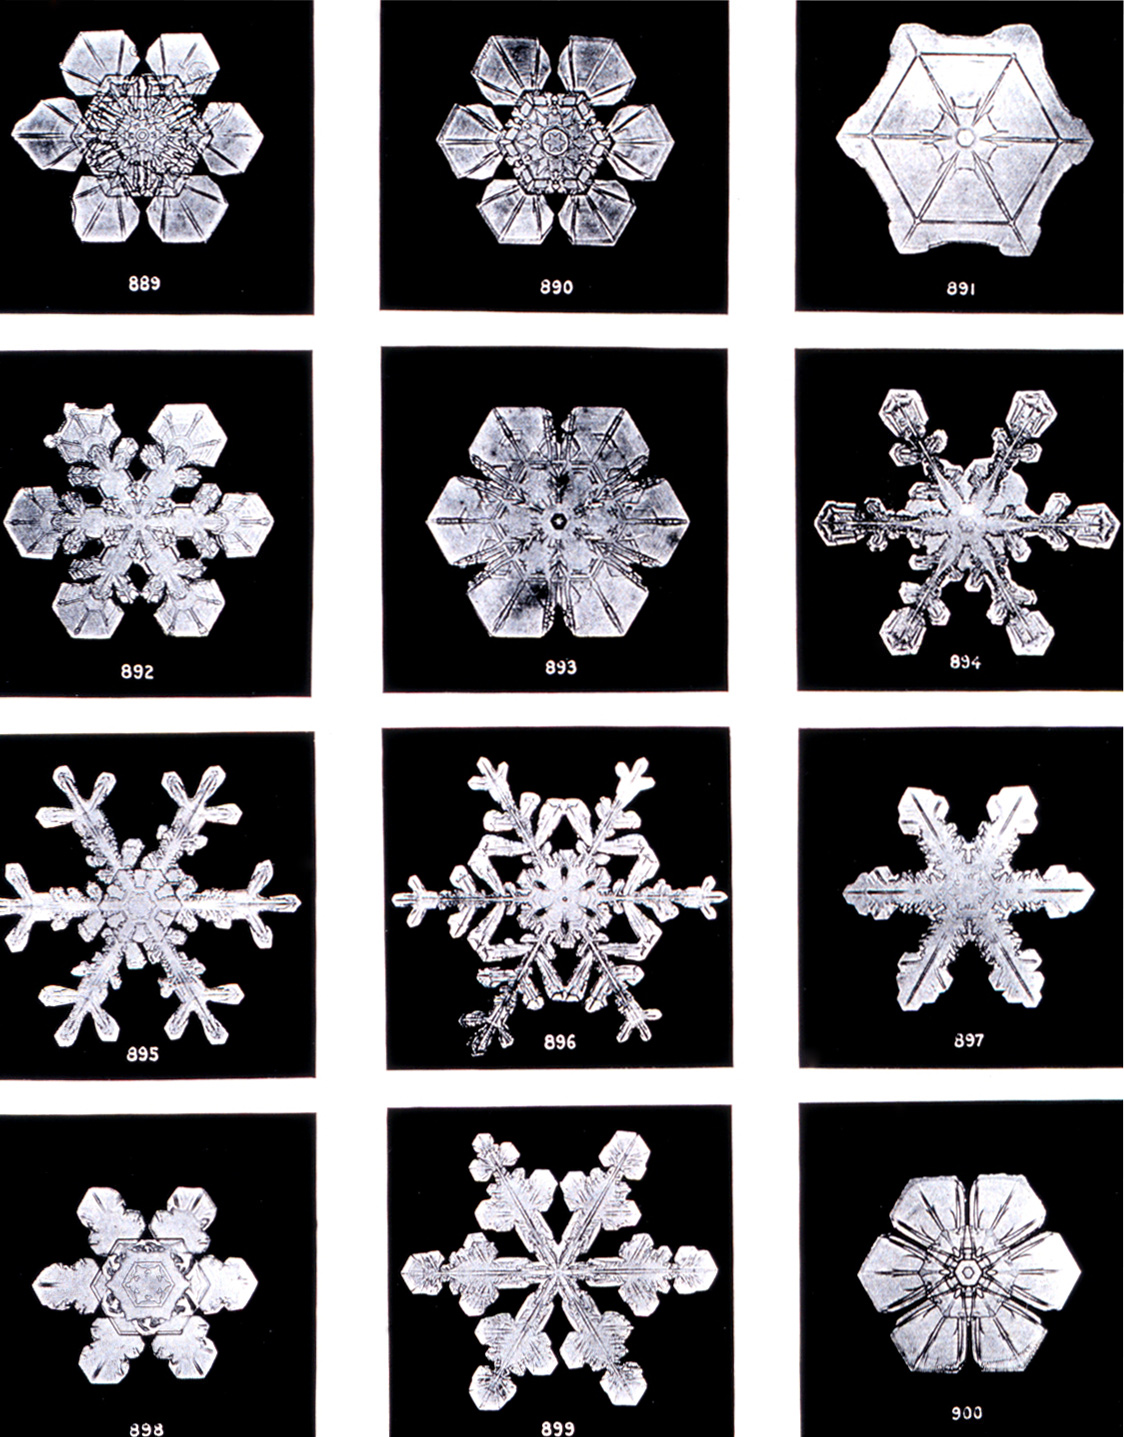
\includegraphics[width=0.36\linewidth]{images/book1/snowflakes.jpg}

{\small Snow crystals photographed by Wilson Bentley in the early 1900s:
every one has six branches.}
\end{omfigure}

\section{Exercises}


\begin{exercise}[$\star$]\label{exo:g11:polarity-and-cohesion:1}
In the bonds \ce{H-Cl}, \ce{O-H} and \ce{C-O}, which \omterm{def:g7:atoms-and-molecules:atom}{atom} carries the
\omterm{def:g11:polarity-and-cohesion:polar-bond}{partial charge} $\delta^-$? Use the table of electronegativities.
\end{exercise}

\begin{exercise}[$\star$]\label{exo:g11:polarity-and-cohesion:2}
Which of these bonds are polar: \ce{H-H}, \ce{C-H}, \ce{O-H}, \ce{N-H},
\ce{Cl-Cl}, \ce{C-Cl}? Give the difference of electronegativities for
each.
\end{exercise}

\begin{exercise}[$\star$]\label{exo:g11:polarity-and-cohesion:3}
Which element is the more electronegative in each pair: nitrogen or
phosphorus; oxygen or sulfur; carbon or nitrogen; sodium or magnesium?
Which trend of the table does each pair illustrate?
\end{exercise}

\begin{exercise}[$\star$]\label{exo:g11:polarity-and-cohesion:4}
Which of \ce{CH4}, \ce{NH3}, \ce{H2O} and \ce{HCl} can form \omterm{def:g11:polarity-and-cohesion:hydrogen-bond}{hydrogen bonds}
between their own \omterm{def:g7:atoms-and-molecules:molecule}{molecules}? Explain.
\end{exercise}

\begin{exercise}[$\star$]\label{exo:g11:polarity-and-cohesion:5}
Are there any attractions between the \omterm{def:g11:polarity-and-cohesion:polar-molecule}{non-polar molecules} of methane?
Why is methane nevertheless a gas at room temperature?
\end{exercise}

\begin{exercise}[$\star\star$]\label{exo:g11:polarity-and-cohesion:6}
Say whether each \omterm{def:g7:atoms-and-molecules:molecule}{molecule} is polar: dichloromethane \ce{CH2Cl2}
(tetrahedral), tetrachloromethane \ce{CCl4}, ammonia \ce{NH3}, carbon
dioxide \ce{CO2}, boron trifluoride \ce{BF3} (a flat triangle with
boron at the centre).
\end{exercise}

\begin{exercise}[$\star\star$]\label{exo:g11:polarity-and-cohesion:7}
In methanol, \ce{CH3-OH}, which hydrogen \omterm{def:g7:atoms-and-molecules:atom}{atom} can be given in a \omterm{def:g11:polarity-and-cohesion:hydrogen-bond}{hydrogen
bond}? Which \omterm{def:g7:atoms-and-molecules:atom}{atom} can receive one? Can methanol and water \omterm{def:g7:atoms-and-molecules:molecule}{molecules} form
\omterm{def:g11:polarity-and-cohesion:hydrogen-bond}{hydrogen bonds} with each other? Draw one.
\end{exercise}

\begin{exercise}[$\star\star$]\label{exo:g11:polarity-and-cohesion:8}
Explain why the boiling temperatures rise in the order \ce{CH4} <
\ce{SiH4} < \ce{GeH4}.
\end{exercise}

\begin{exercise}[$\star\star$]\label{exo:g11:polarity-and-cohesion:9}
On the chart of the boiling temperatures of the hydrides, which group
shows no unusual value for its first member? Why?
\end{exercise}

\begin{exercise}[$\star\star$]\label{exo:g11:polarity-and-cohesion:10}
% ledger: en:H, en:Cl, en:Br, en:I, bp:HCl, bp:HBr, bp:HI
The bonds \ce{H-Cl}, \ce{H-Br}, \ce{H-I} are less and less polar (the
electronegativities of chlorine, bromine and iodine are 3.16, 2.96 and
2.66), yet the boiling temperatures rise: \qty{-85}{\celsius},
\qty{-66}{\celsius}, \qty{-35}{\celsius}. Which interaction wins, and
why?
\end{exercise}

\begin{exercise}[$\star\star$]\label{exo:g11:polarity-and-cohesion:11}
At room temperature chlorine is a gas and iodine a solid, though both
are made of \omterm{def:g11:polarity-and-cohesion:polar-molecule}{non-polar molecules} \ce{X2}. Explain.
\end{exercise}

\begin{exercise}[$\star\star\star$]\label{exo:g11:polarity-and-cohesion:12}
% ledger: bp:C2H5OH, bp:CH3OCH3, bp:C3H8
Ethanol \ce{CH3-CH2-OH}, methoxymethane \ce{CH3-O-CH3} and propane
\ce{CH3-CH2-CH3} have nearly the same \omterm{def:g10:the-mole:molar-mass}{molar mass}. They boil at
\qty{78}{\celsius}, \qty{-25}{\celsius} and \qty{-42}{\celsius}. Which
of them are polar? Which form \omterm{def:g11:polarity-and-cohesion:hydrogen-bond}{hydrogen bonds} between their own
\omterm{def:g7:atoms-and-molecules:molecule}{molecules}? Explain the order.
\end{exercise}

\begin{exercise}[$\star\star\star$]\label{exo:g11:polarity-and-cohesion:13}
In ice each water \omterm{def:g7:atoms-and-molecules:molecule}{molecule} is hydrogen-bonded to four neighbours, in an
open network; in liquid water the network keeps breaking and partly
collapses. Explain why ice floats on water. Why is this important for
the fish of a frozen lake?
\end{exercise}

\begin{exercise}[$\star\star\star$]\label{exo:g11:polarity-and-cohesion:14}
Sort in increasing order of melting temperature, and justify by the
attractions between the particles: potassium chloride \ce{KCl}, ice
\ce{H2O}, solid methane \ce{CH4}.
\end{exercise}

\begin{exercise}[$\star\star\star$]\label{exo:g11:polarity-and-cohesion:15}
% ledger: en:F, en:O, bp:HF, bp:H2O
Fluorine is more electronegative than oxygen, so an \ce{H-F} bond is
more polar than an \ce{O-H} bond. Yet water boils at \qty{100}{\celsius}
and hydrogen fluoride at \qty{20}{\celsius}. Count the hydrogen \omterm{def:g7:atoms-and-molecules:atom}{atoms}
each \omterm{def:g7:atoms-and-molecules:molecule}{molecule} can give and the \omterm{def:g10:lewis-and-shape:lone-pair}{lone pairs} it can receive with, and
explain.
\end{exercise}

\section{Problem: Why Does Water Boil at \texorpdfstring{\qty{100}{\celsius}}{100 degrees Celsius}?}

\begin{problem}[{Weekend problem --- without hydrogen bonds, at what
temperature would water boil?}]
\label{pb:g11:polarity-and-cohesion:1}
% ledger: en:H, en:O, en:S, en:Se, bp:H2O, bp:H2S, bp:H2Se, bp:CH4, bp:SiH4, bp:GeH4, bp:HCl, bp:HBr, bp:HF, bp:NH3, bp:PH3, bp:AsH3
Oxygen, sulfur and selenium are in the same group of the table, and all
three form a compound with hydrogen: \ce{H2O}, \ce{H2S}, \ce{H2Se}. In
each group of hydrides, boiling temperatures usually rise with the size
of the \omterm{def:g7:atoms-and-molecules:molecule}{molecule}. Water breaks the rule. By how much?

\medskip
\noindent\textbf{Part I --- Three \omterm{def:g7:atoms-and-molecules:molecule}{molecules}.}
\begin{enumerate}
  \item Draw the \omterm{def:g10:lewis-and-shape:lewis-structure}{Lewis structures} of \ce{H2O}, \ce{H2S} and \ce{H2Se}.
        Why are they alike?
  \item Compute their molar masses.
  \item Compute the differences of \omterm{def:g11:polarity-and-cohesion:electronegativity}{electronegativity} of the bonds
        \ce{O-H}, \ce{S-H} and \ce{Se-H} (oxygen 3.44, sulfur 2.58,
        selenium 2.55, hydrogen 2.20). Which bonds are clearly polar?
  \item What is the shape of the three \omterm{def:g7:atoms-and-molecules:molecule}{molecules}? Are they polar?
  \item Count the \omterm{def:g9:inside-the-atom:nucleus}{electrons} of each \omterm{def:g7:atoms-and-molecules:molecule}{molecule}. Which has the strongest \omterm{def:g11:polarity-and-cohesion:van-der-waals}{van
        der Waals interactions}?
\end{enumerate}

\medskip
\noindent\textbf{Part II --- \omterm{def:g11:polarity-and-cohesion:hydrogen-bond}{Hydrogen bonds}.}
\begin{enumerate}[resume]
  \item Which of the three compounds forms \omterm{def:g11:polarity-and-cohesion:hydrogen-bond}{hydrogen bonds} between its
        \omterm{def:g7:atoms-and-molecules:molecule}{molecules}? Why not the others?
  \item How many \omterm{def:g11:polarity-and-cohesion:hydrogen-bond}{hydrogen bonds} can one water \omterm{def:g7:atoms-and-molecules:molecule}{molecule} take part in at
        most? Draw them.
  \item Which interactions hold the \omterm{def:g7:atoms-and-molecules:molecule}{molecules} of hydrogen sulfide
        together in the liquid?
\end{enumerate}

\medskip
\noindent\textbf{Part III --- The trend.}
\begin{enumerate}[resume]
  \item Hydrogen sulfide boils at \qty{212.9}{K} and hydrogen selenide at
        \qty{-41.3}{\celsius}. Express the first in degrees Celsius
        ($\theta = T - 273.15$).
  \item By how much does the boiling temperature rise from period 3
        (\ce{H2S}) to period 4 (\ce{H2Se})?
  \item Why does it rise?
  \item Assuming the same rise from period 2 to period 3, at what
        temperature would a ``normal'' \ce{H2O} boil?
  \item Test the method on \omterm{def:g9:periodic-table-first-look:period}{group} 14: \ce{SiH4} boils at
        \qty{-112}{\celsius} and \ce{GeH4} at \qty{-88.1}{\celsius}.
        Predict the boiling temperature of \ce{CH4} and compare with the
        real one, \qty{-162}{\celsius}. Is the extrapolation exact?
  \item Do the same for \omterm{def:g9:periodic-table-first-look:period}{group} 17 (\ce{HCl} \qty{-85.1}{\celsius},
        \ce{HBr} \qty{-66.4}{\celsius}) and compare with \ce{HF},
        \qty{19.6}{\celsius}.
\end{enumerate}

\medskip
\noindent\textbf{Part IV --- The gap.}
\begin{enumerate}[resume]
  \item Water really boils at \qty{100}{\celsius}. How large is the gap
        between the real and the extrapolated values?
  \item Same for ammonia, using \ce{PH3} \qty{-87.8}{\celsius} and
        \ce{AsH3} \qty{-62.5}{\celsius}; ammonia really boils at
        \qty{-33.4}{\celsius}.
  \item Rank water, hydrogen fluoride and ammonia by the size of their
        gap, and explain the ranking by counting \omterm{def:g11:polarity-and-cohesion:hydrogen-bond}{hydrogen bonds}.
  \item Without \omterm{def:g11:polarity-and-cohesion:hydrogen-bond}{hydrogen bonds}, would water be a solid, a liquid or a gas
        at room temperature? What would that mean for the Earth?
  \item Why is the answer of question 12 only an estimate?
  \item State the final answer: at about what temperature would water
        boil without \omterm{def:g11:polarity-and-cohesion:hydrogen-bond}{hydrogen bonds}?
\end{enumerate}
\end{problem}
